\chapter{Mapping the Data}
\label{ch:mapping-the-data}

Imagine a foreign visitor to the US who knows nothing about the US geography. He doesn't even have a map; the only data he has is a list of distances between the cities. Oh, yes, and he attended the Introduction to Data Mining.

If we know distances between the cities, we can cluster them.\marginnote{For this example we retrieved the data from \url{http://www.mapcrow.info/united_states.html}, removed the city names from the first line and replaced it with "31 labelled".\break\break The file is available at \url{http://file.biolab.si/files/us-cities.dst.zip}. To load it, unzip the file and use the \widget{File Distance} widget.}

\begin{figure}[h]
    \centering
    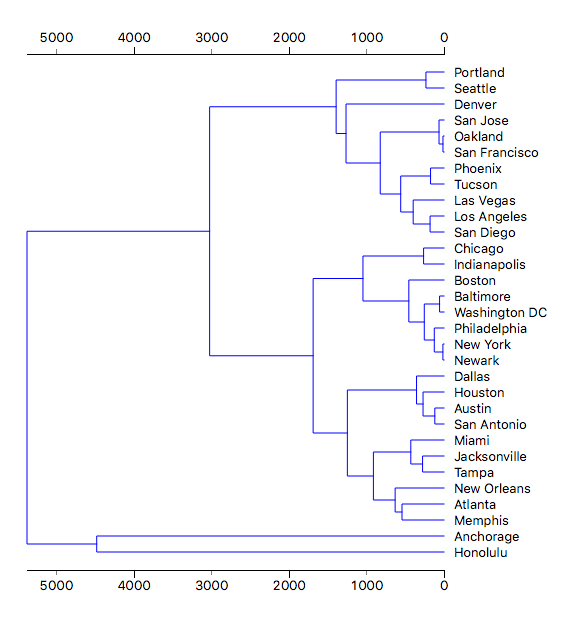
\includegraphics[width=\linewidth]{dendrogram.png}
    \caption{$\;$}
\end{figure}

How much sense does it make? Austin and San Antonio are closer to each other than to Houston; the tree is then joined by Dallas. On the other hand, New Orleans is much closer to Houston than to Miami. And, well, good luck hitchhiking from Anchorage to Honolulu.

As for Anchorage and Honolulu, they are leftovers; when there were only three clusters left (Honolulu, Anchorage and the big cluster with everything else), Honolulu and Anchorage were closer to each other than to the rest. But not close — the corresponding lines in the dendrogram are really long.

The real problem is New Orleans and San Antonio: New Orleans is close to Atlanta and Memphis, Miami is close to Jacksonville and Tampa. And these two clusters are suddenly more similar to each other than to some distant cities in Texas.

\marginnote{We can't run k-means clustering on this data, since we only have distances, and k-means runs on real (tabular) data. Yet, k-means would have the same problem as hierarchical clustering.}In general, two points from different clusters may be more similar to each other than to some points from their corresponding clusters.

To get a better impression about the physical layout of cities, people have invented a better tool: a map! Can we reconstruct a map from a matrix of distances? Sure. Take any pair of cities and put them on a paper with the distance corresponding to some scale. Add the third city and put it at the corresponding distance from the two. Continue until done. Excluding, for the sake of scale, Anchorage, we get the following map.

\begin{figure*}[h]
    \centering
    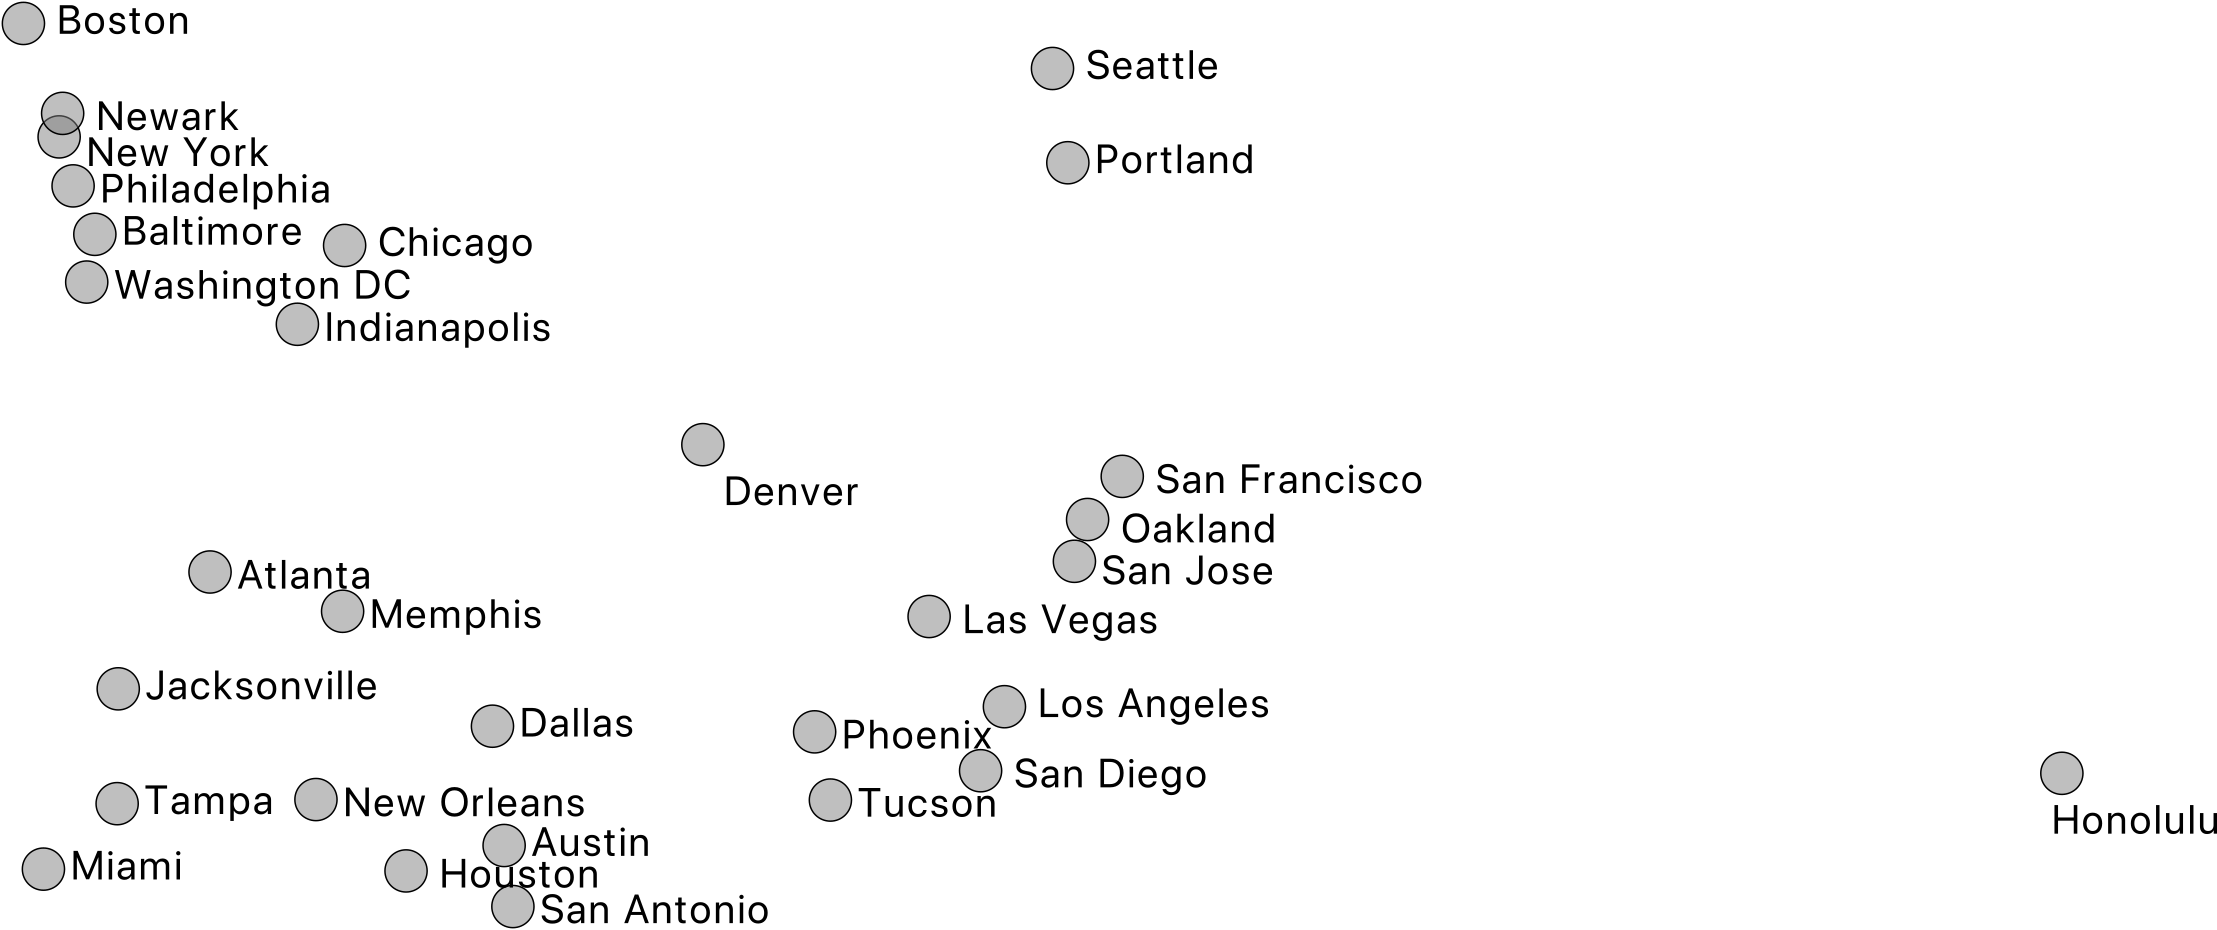
\includegraphics[width=\linewidth]{mds-jitter.png}
    \caption{$\;$}
\end{figure*}

We have not constructed this map manually, of course. We used a widget called \widget{MDS}, which stands for Multidimensional scaling.

It is actually a rather exact map of the US from the Australian perspective. You cannot get the orientation from a map of distances, but now we have a good impression about the relations between cities. It is certainly much better than clustering.

\begin{marginfigure}
    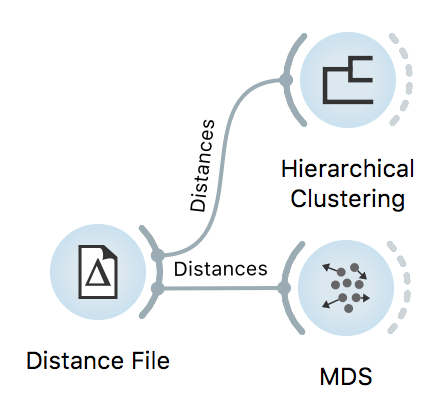
\includegraphics[width=\linewidth]{distance-workflow.png}
\end{marginfigure}

\newpage

Remember the clustering of animals? Can we draw a map of animals?
Does the map make any sense? Are similar animals together? Color the points by the types of animals and you should see.

\begin{figure}[h]
    \centering
    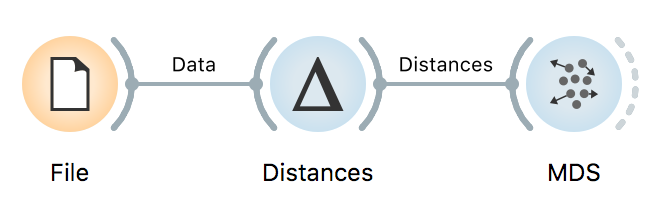
\includegraphics[scale=0.7]{zoo-workflow.png}
    \caption{$\;$}
\end{figure}

\begin{figure*}[h]
    \centering
    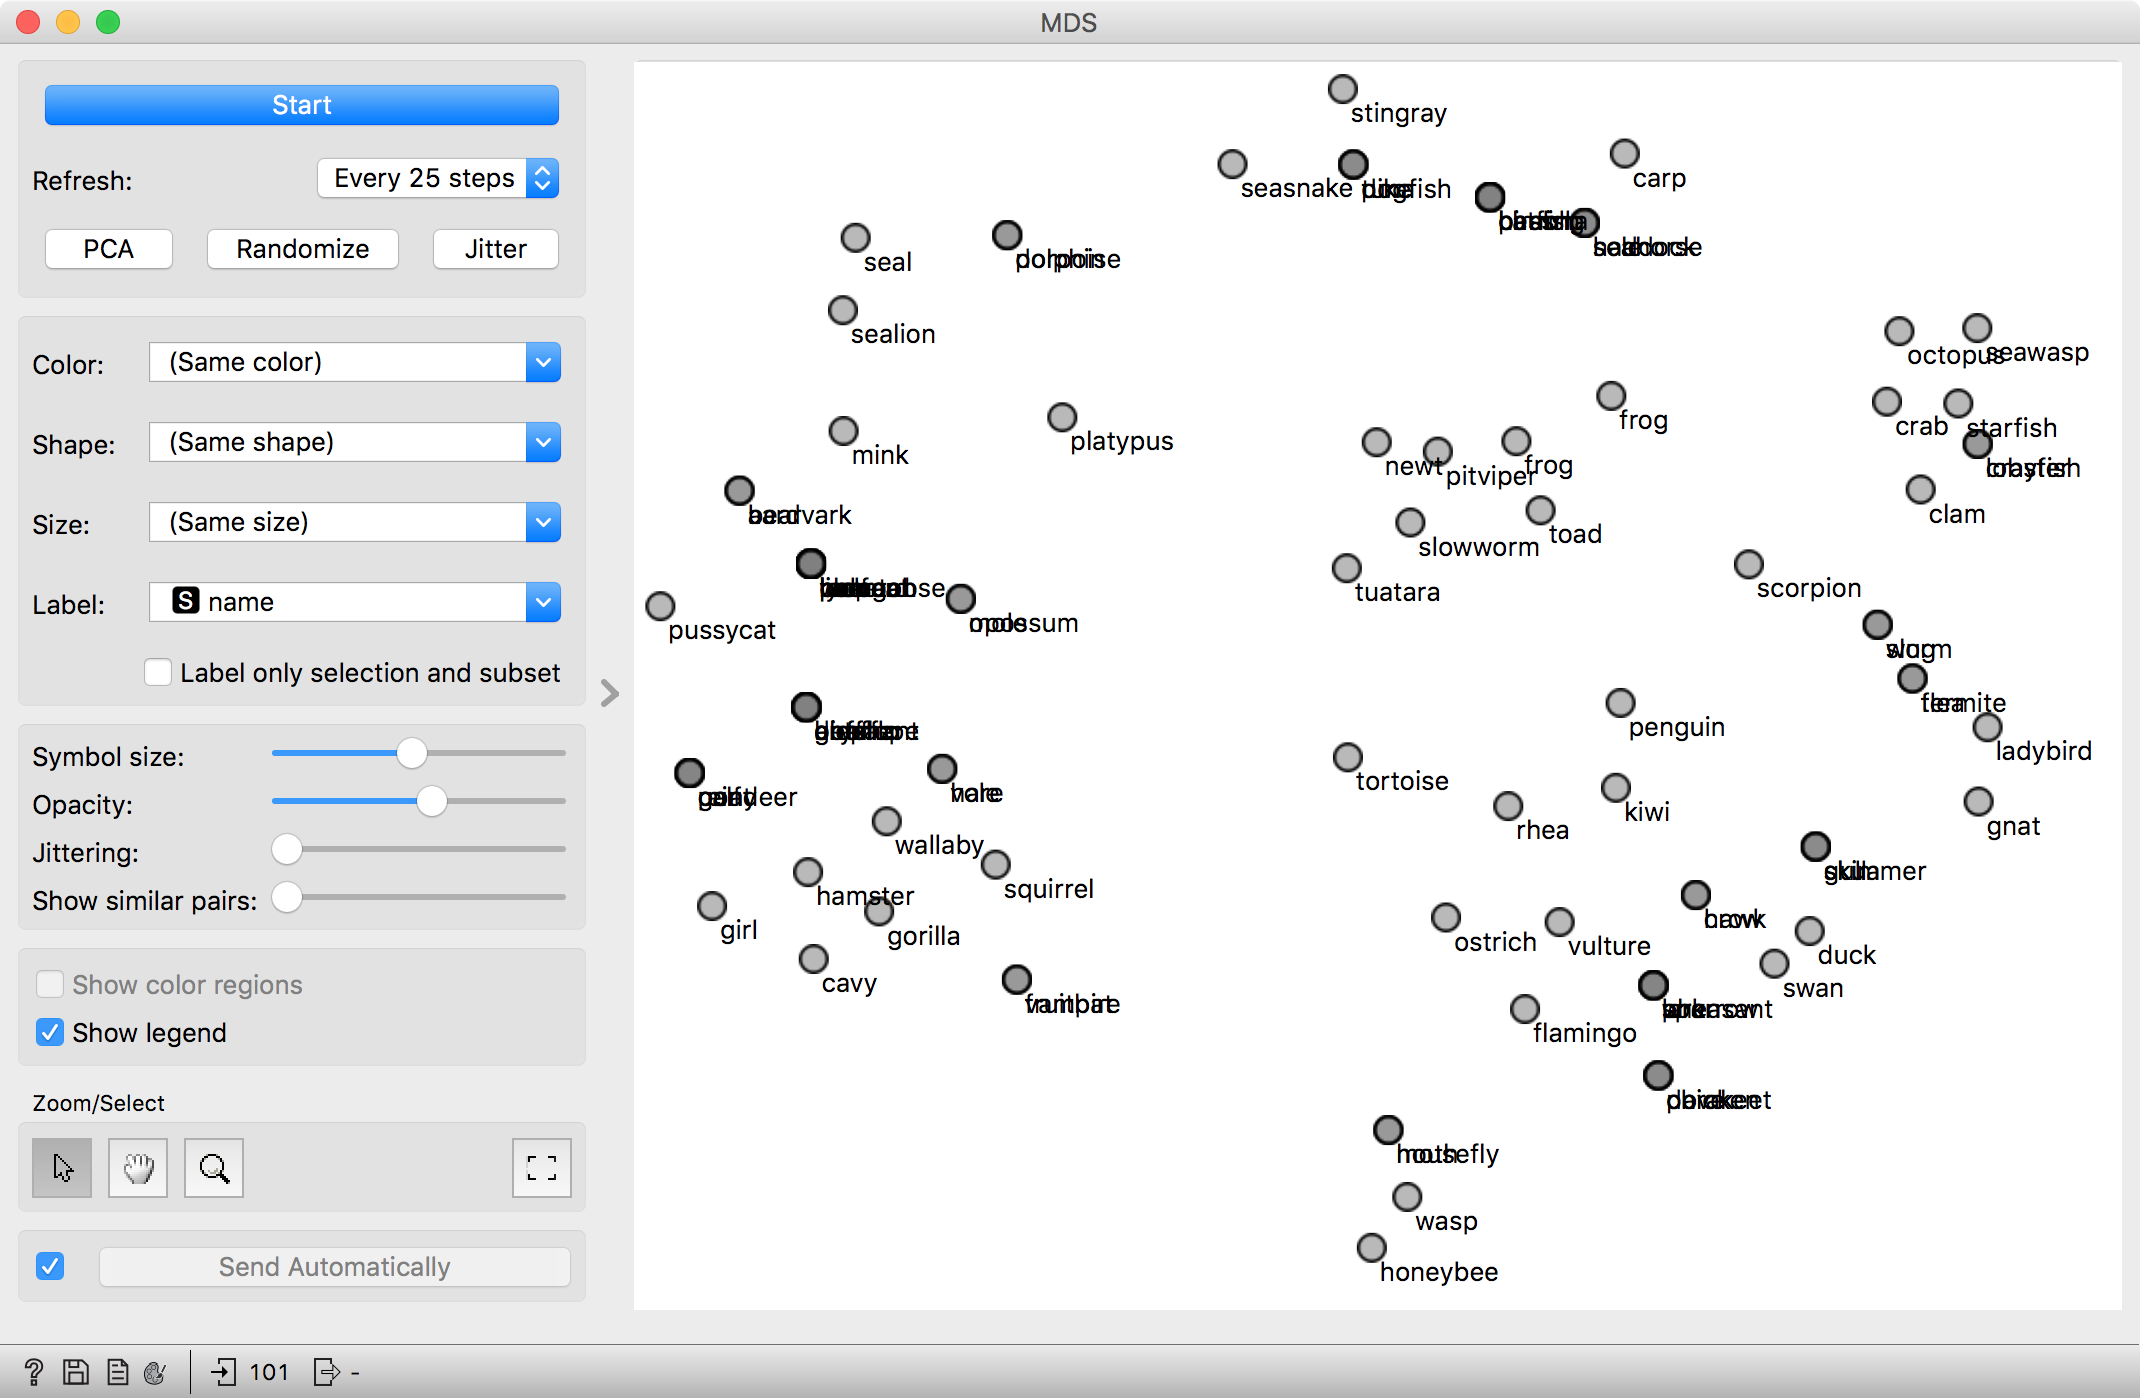
\includegraphics[width=\linewidth]{zoo-mds.png}
    \caption{$\;$}
\end{figure*}

The map of the US was accurate: one can put the points in a plane so that the distances correspond to actual distances between cities. For most data, this is usually impossible. What we get is a projection (a non-linear projection, if you care about mathematical finesses) of the data. You lose something, but you get a picture.

The MDS algorithm does not always find the optimal map. You may want to restart the MDS  from random positions. Use the slider "Show similar pairs" to see whether the points that are placed together (or apart) actually belong together. In the above case, the honeybee belongs closer to the wasp, but could not fly there as in the process of optimization it bumped into the hostile region of flamingos and swans.
